\documentclass[../main.tex]{subfiles}
\begin{document}

As part of our project, we implemented two fully instrumented FaaS based demo applications:
An e-commerce application (i.e.\@ a webshop) and an IoT-resembling traffic light calculator for some road crossing.
They serve both as examples how to build fully working and adaptively deployable applications 
within our framework as well as a baseline for real application-oriented FaaS benchmarks.

\section{E-Commerce Application (Webshop)}\label{sec:webshop}

% Design Concepts
We implemented a test e-commerce application that fully consists of FaaS components together with a redis database. 
The basic functionality is to display recommended products and ads to customers 
who can then buy said products by charging a mocked credit card. 
As such, the deployed application can theoretically be ``used'' exclusively by humans 
interacting with its website frontend within a web browser.
Naturally, there are also pre-defined automized workloads to secure a benchmark's reproducibility.

The whole functionality is closely oriented on Google’s microservices demo v0.1.0\footnotemark{} 
but has of course been fully reimplemented as a FaaS project (except some HTML templates as referenced within their code directory). 
\footnotetext{\url{https://github.com/GoogleCloudPlatform/microservices-demo/tree/bae651f7ea537d2676b38a04d89adacdd45c17bd}}

\subsection{Application Structure}\label{ssec:webshopApplicationStructure}

\begin{figure}
\begin{center}
  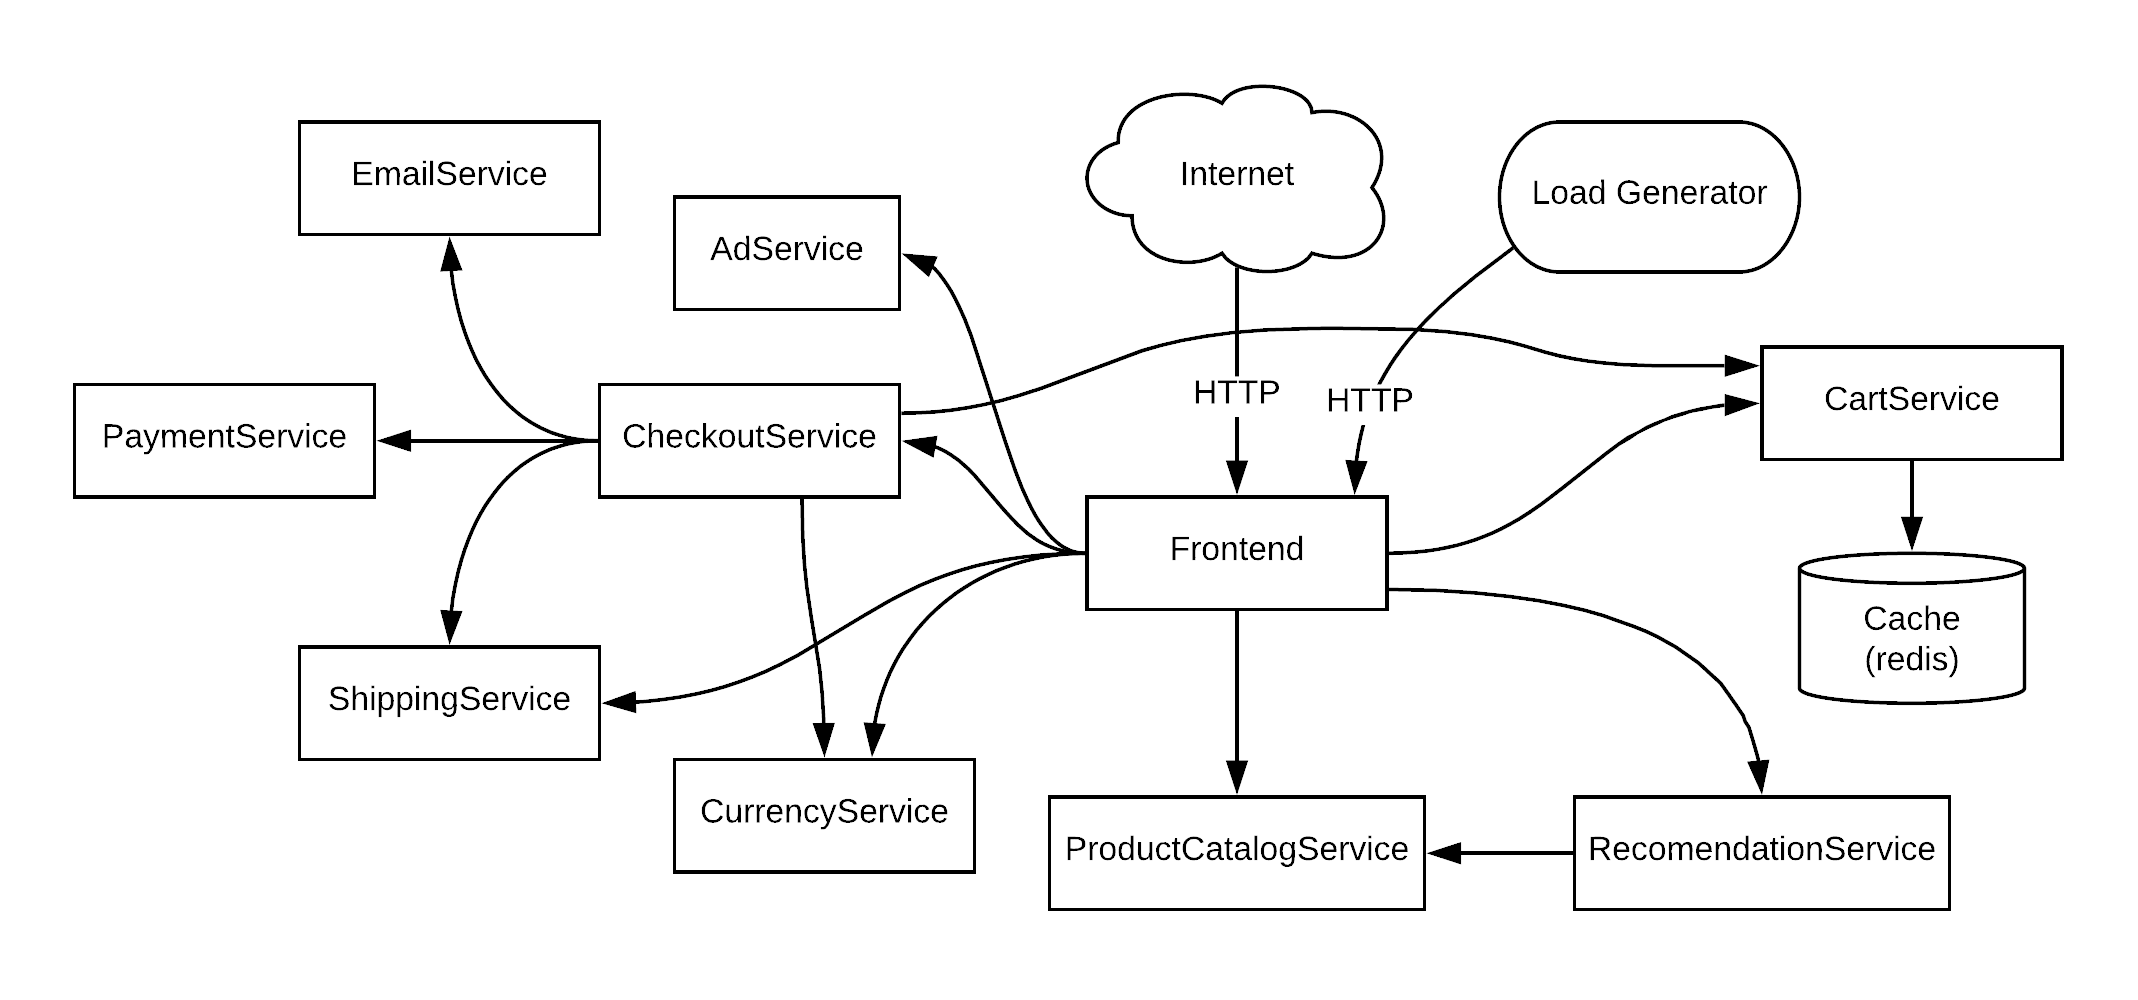
\includegraphics[width=\linewidth,keepaspectratio]{./webshop-architecture-diagram.png}
\end{center}
\caption[Webshop Architecture Diagram]{%
  Webshop architecture diagram as illustrated by Google\protect\footnotemark.
  %TODO remove external API
  All `services' as well as the frontend are implemented as one function within our demo application. 
  They communicate internally with each other via our library's RPC system and are thus automatically measured at runtime.%
}%
\label{fig:webshopArchitectureDiagram}
\end{figure}
\footnotetext{\url{https://raw.githubusercontent.com/GoogleCloudPlatform/microservices-demo/bae651f7ea537d2676b38a04d89adacdd45c17bd/docs/img/architecture-diagram.png}}


\subsection{Benchmarking Properties}\label{ssec:webshopApplicationProperties}


\subsection{Specific Workloads}\label{ssec:webshopSpecificWorkloads}


\end{document}
